\chapter{Türerkennung}

Die Türerkennung erfolgt in mehreren Schritten. Zuerst, wird im Bild nach Kanten gesucht. Die gefundenen Kanten müssen hinsichtlich Länge und Ausrichtung optimiert werden. Anschliessend muss nach möglichen Vier-Kanten-Paaren gesucht werden, welche möglicherweise eine Tür bilden. Die gefundenen Kandidaten werden dann noch evaluiert, um den besten Treffer zu bestimmen.

\section{Kantendetektion}

Es existieren verschiedene Algorithmen um Kanten in Bildern zu suchen. In dieser Arbeit wurden speziell die "Probabilistic Hough-Line-Transformation" und die "Line Segment detection using Weighted Mean-Shift" oder kurz LSWMS untersucht. Beide sind darauf spezialisiert Geraden zu finden, wobei es merkliche Unterschiede zwischen den zwei Methoden gibt.

\subsection{Probabilistic Hough-Line-Transformation}

\subsection{LSWMS}

\subsection{Evaluation}

Die Entscheidung fiel auf den LSWMS Algorithmus, aus mehreren Gründen. LSWMS wurde von Anfang an für die unbeaufsichtigte Kantendetektion innerhalb von Echtzeitanwendungen konzipiert. Da die Umgebungen in denen die Türdetektion stattfindet stark variieren können, ist es nicht möglich im vorhinein fixe Parameter für die Hough-Transformation zu definieren, welche überall gleich gut funktionieren. LSWMS bietet im Schnitt unter sich verändernden Verhältnissen die bessere Leistung.
\paragraph{}
Ein weiterer Faktor ist die Qualutät der zurückgegebenen Resultate. Die Anzahl fehlerhaft erkannten Kanten ist bei Hough erheblich höher als bei LSWMS und wirkt sich damit auch auf die Performance der weiteren Verarbeitungsschritte negativ aus. Die Möglichkeit bei LSWMS eine Obergrenze bezüglich der Anzahl erwarteter Treffer angeben zu können war ebenfalls ausschlaggebend. Bei "ruhigen" Bildern mit wenig potentiellen Kanten wirkt sich dies wenig aus. Bilder welche z.B. Türem mit Holzmuster enthalten führen bei Hough zu einer Fehlerquote von teilweise über 50\%.
\paragraph{}
Der letzte Faktor welcher zur Entscheidung geführt hat LSWMS vorzuziehen war die Gesamtperformance. Hough benötigt als Input ein Kantenbild, welches zuvor mit einem separaten Algorithmus aufgearbeitet werden muss, z.B. Canny\footnote{\protect\url{http://de.wikipedia.org/wiki/Canny-Algorithmus}}. Dieser Schritt führt zusätzliche Parameter ein, welche situationsbedingt optimiert werden müssen und erhöht die Verarbeitungszeit der Hough-Transformation. Da Canny empfindlich gegenüber Rauschen im Bildmaterial ist, muss ein weiterer Verarbeitungsschritt vorangestellt werden. Bevor Canny angewendet wird, werden mittels einem Gausschen Filter Störfaktoren reduziert. Um ein optimales Ergebnis zu erhalten müssen vertikale und horizontale Kanten separat gesucht werden. Dies hat zu folge das die Hough-Transformation zwei mal dürchgeführt werden muss (Canny muss nur einmal angewendet werden, beide Male kann das selbe Kantenbild verwendet werden).
\paragraph{}
Für den Vergleich der Hough-Transformation und LSWMS wurden folgende Parameter verwendet:
\paragraph{}
Gauss Filter (medianBlur)\footnote{\protect\url{http://docs.opencv.org/modules/imgproc/doc/filtering.html?highlight=medianblur#medianblur}}
\begin{itemize}
	\item kSize: 5
\end{itemize}
Canny Edge Detection\footnote{\protect\url{http://docs.opencv.org/doc/tutorials/imgproc/imgtrans/canny_detector/canny_detector.html}}
\begin{itemize}
	\item lowThreshold: 20
	\item highThreshold: 80
	\item kernelSize: 3
\end{itemize}
Probabilistic Hough-Line-Transformation\footnote{\protect\url{http://docs.opencv.org/doc/tutorials/imgproc/imgtrans/hough_lines/hough_lines.html}}
\begin{itemize}
	\item rho: 1
	\item theta: 1 rad
	\item threshold: 80
	\item minLinLength: 30
	\item maxLineGap: 10
\end{itemize}
LSWMS
\begin{itemize}
	\item numMaxLSegs: 1000
\end{itemize}

Die gelben Linien stellen die gefundenen Kanten bzw. Kanstensegmente dar.
\pagebreak

\begin{figure}[!ht]
\centering
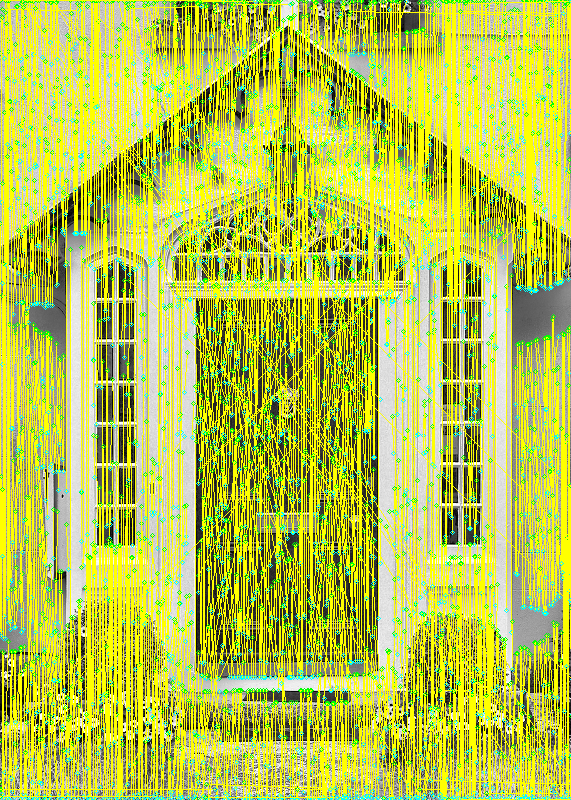
\includegraphics[scale=0.6]{images/hough-raw-segments} 
\caption{Ergebnis Hough-Transformation}
\label{fig:hough-raw-segments}
\end{figure}

\pagebreak

\begin{figure}[!ht]
\centering
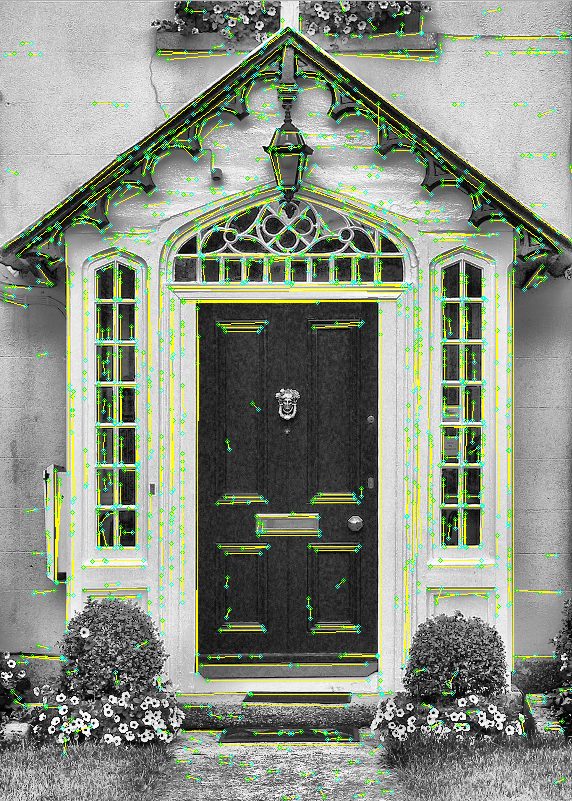
\includegraphics[scale=0.6]{images/lswms-raw-segments} 
\caption{Ergebnis LSWMS}
\label{fig:hough-raw-segments}
\end{figure}

\pagebreak

Dies ist nur ein Bild von zehn getesteten. Die Bilder welche während der Entwicklung zum Testen verwendet wurden können im Projektverzeichnis unter Data/Images/Doors/Misc gefunden werden. Es ist klar ersichtlich, dass LSWMS das qualitativ bessere Ergebnis liefert. Einziger Nachteil hier ist, dass LSWMS oft nicht durgehende Kanten erkennt sondern kleinere Segmente entlang der Kante zurückgibt. Neben der Qualität der Resultate wurde auch die Performance beider Methoden analysiert. Da einige Testbilder grösser sind als in der finalen Applikation benötigt, wurden alle Bilder auf eine Höhe von 800 Pixel verkleinert. Nachfolgend das Ergebnis (Durchschnitt aus 100 Durchgängen):

\begin{itemize}
	\item Hough: 165ms, 1871 Segmente
	\item LSWMS: 64ms, 868 Segmente
\end{itemize}

Auch hier ist LSWMS Hough überlegen. Obwohl LSWMS für Echtzeitanwendungen konzipiert wurde, kann mit den gemessenen 64ms Verarbeitungszeit pro Frame kein flüssiges Videobild bei 28fps wiedergegeben werden.

\section{Implementation}

\begin{figure}
	\subfloat[Segmente wie sie mit LSWMS gefunden werden]{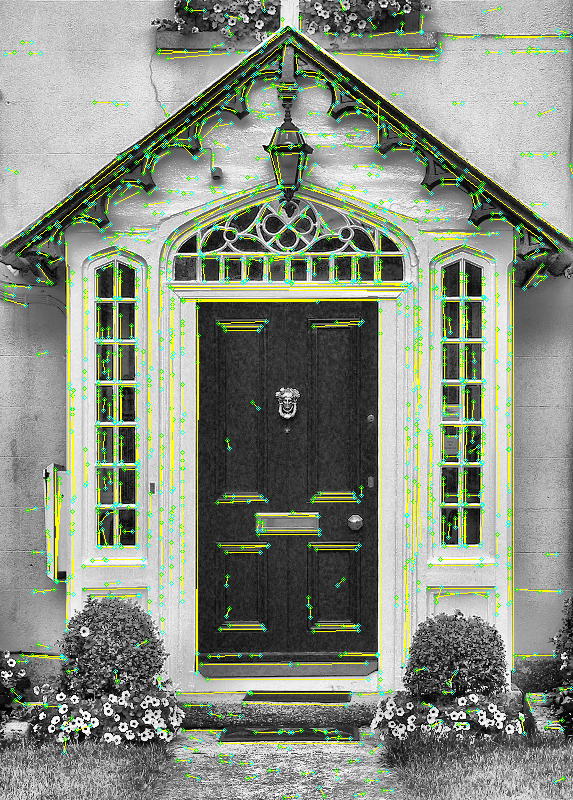
\includegraphics[width=0.45\textwidth]{images/seg-raw}}\qquad	
	\subfloat[Segmente kategorisiert in horizontal (Rot) und vertikal (Gelb)]{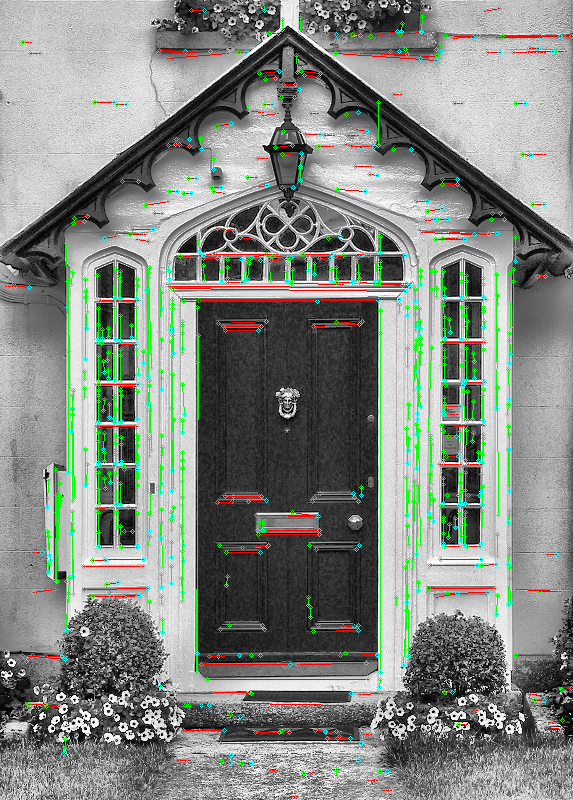
\includegraphics[width=0.45\textwidth]{images/seg-categorized}}\qquad	
	\subfloat[Reduzierte Segmente]{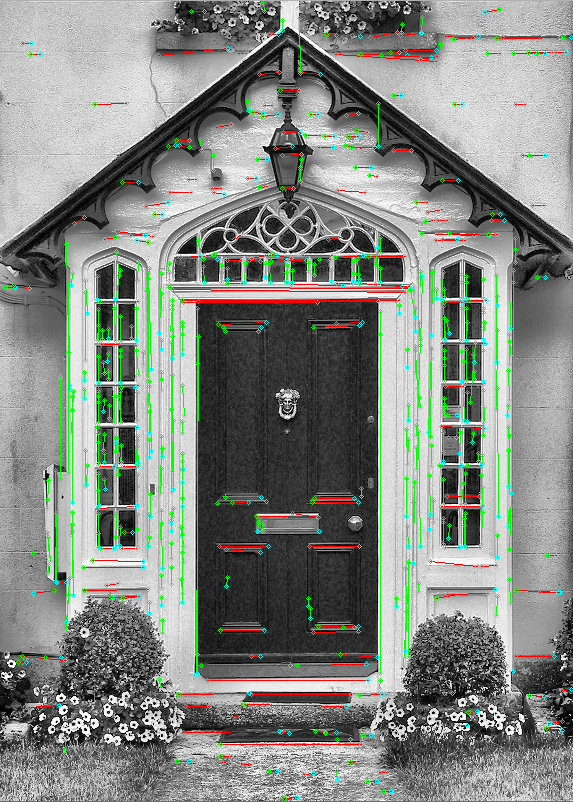
\includegraphics[width=0.45\textwidth]{images/seg-joined}}	\qquad	
	\subfloat[Verlängerte Segmente]{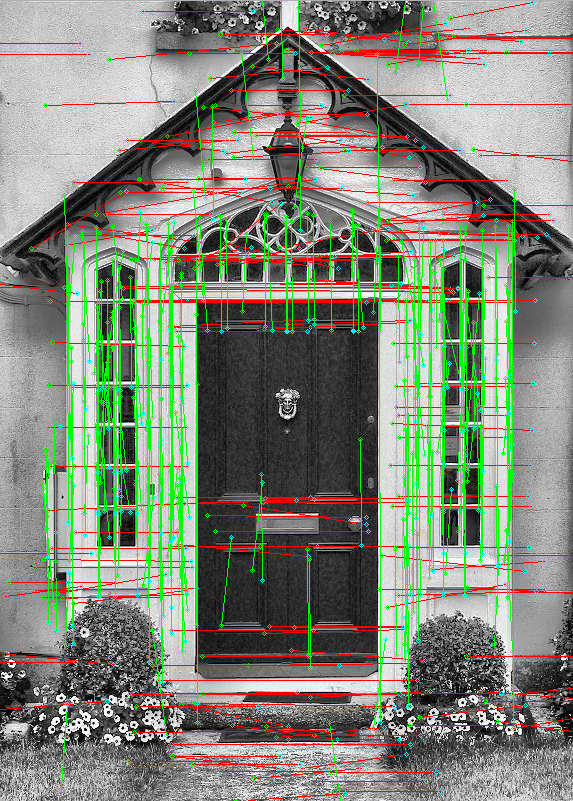
\includegraphics[width=0.45\textwidth]{images/seg-grow}}	
	\caption{Verarbeitungsprozess Türerkennung}
\end{figure}

\begin{figure}
	\ContinuedFloat
	\centering		
	
	\subfloat[Erkannte Tür]{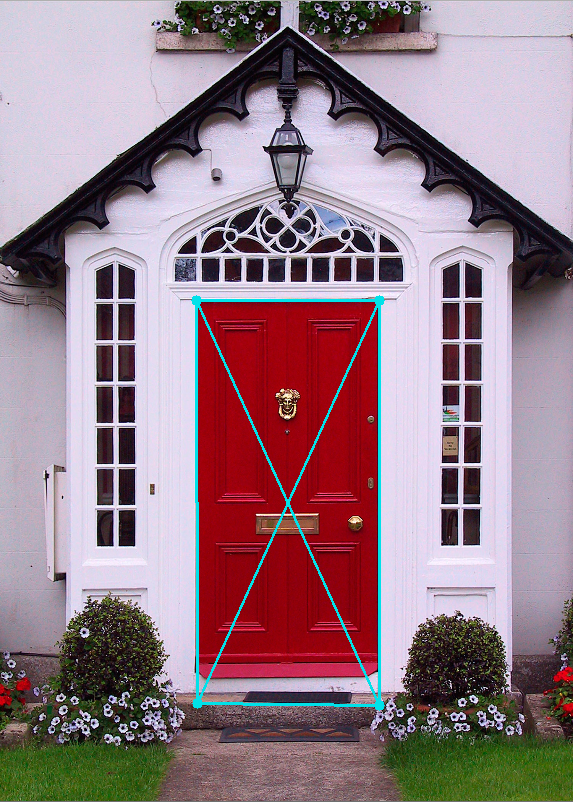
\includegraphics[width=0.45\textwidth]{images/seg-detected}}\qquad
	\caption{Verarbeitungsprozess Türerkennung}
\end{figure}

\subsection{Performance}

\subsection{Verbesserungsmöglichkeit}